
\documentclass[UTF8]{article}
\usepackage{xeCJK}
\usepackage{amsmath,amssymb}
\begin{document}

   \chapter{Operating system interfaces}   
    \label{CH:UNIX}     

操作系统的工作是在多个程序之间共享计算机,并提供比硬件单独支持的更有用的服务集。操作系统管理和抽象低级硬件,因此,例如,文字处理器不需要关心正在使用哪种类型的磁盘硬件。操作系统在多个程序之间共享硬件,以便它们同时运行(或看似运行)。最后,操作系统为程序交互提供受控方式,以便它们可以共享数据或协同工作。  

操作系统通过接口向用户程序提供服务。
    \index{interface design}    设计一个好的界面是很困难的。一方面,我们希望界面简单而狭窄,因为这样更容易正确实现。另一方面,我们可能会想为应用程序提供许多复杂的功能。解决这种矛盾的技巧是设计依赖于一些机制的界面,这些机制可以组合起来以提供更多的通用性。  

本书以单个操作系统作为具体例子来说明操作系统概念。该操作系统 xv6 提供了 Ken Thompson 和 Dennis Ritchie 的 Unix 操作系统~    \cite{unix}    引入的基本接口,并模仿了 Unix 的内部设计。 Unix 提供了一个狭窄的接口,其机制结合得很好,提供了令人惊讶的通用性。这种接口非常成功,以至于现代操作系统(BSD、Linux、macOS、Solaris,甚至在较小程度上,Microsoft Windows)都具有类似 Unix 的接口。了解 xv6 是了解这些系统和许多其他系统的良好开端。  

如图〜   \ref{fig:os}   所示,xv6采用传统形式
    \indextext{kernel}    ,一个为正在运行的程序提供服务的特殊程序。每个正在运行的程序,称为
    \indextext{process}    ,具有包含指令、数据和堆栈的内存。这些指令实现程序的计算。数据是计算所作用的变量。堆栈组织程序的过程调用。给定的计算机通常具有许多进程,但只有一个内核。  

当进程需要调用内核服务时,它会调用    \indextext{system call}    ,这是操作系统接口中的调用之一。系统调用进入内核;内核执行服务并返回。因此,一个进程交替执行
    \indextext{user space}    和
    \indextext{kernel space}    。  

正如后续章节中详细描述的,内核使用 CPU    \footnote{本文通常指的是使用术语    \indextext{CPU}    执行计算的硬件元件,   \indextext{CPU}    是中央处理单元的缩写。其他文档(例如 RISC-V 规范)也使用词语“处理器”、“核心”和“hart”来代替“CPU”。  }    提供的硬件保护机制来确保在用户空间中执行的每个进程只能访问自己的内存。内核以实现这些保护所需的硬件权限执行;用户程序在没有这些权限的情况下执行。当用户程序调用系统调用时,硬件会提高特权级别并开始执行内核中预先安排的功能。  

   \begin{figure}[t]
\center
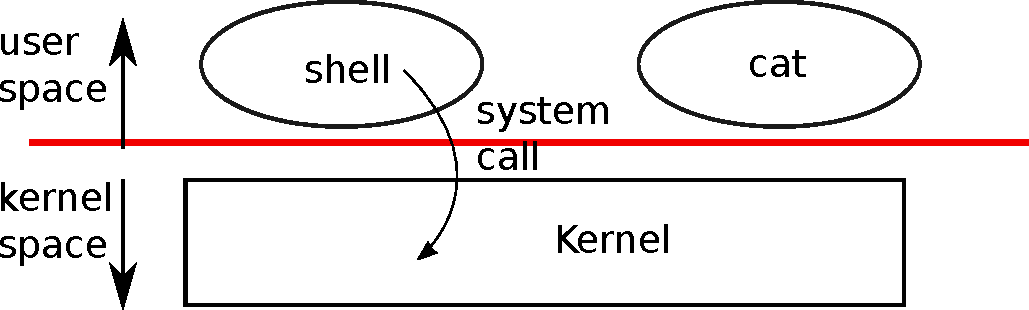
\includegraphics[scale=0.5]{fig/os.pdf}
\caption{一个内核和两个用户进程。  }
\label{fig:os}
\end{figure}     

内核提供的系统调用的集合是用户程序看到的接口。 xv6 内核提供了 Unix 内核传统上提供的服务和系统调用的子集。图~   \ref{fig:api}   列出了xv6的所有系统调用。  

本章的其余部分概述了 xv6 的服务——进程、内存、文件描述符、管道和文件系统——并用代码片段和讨论 Unix 的命令行用户界面    \indextext{shell}    如何使用它们来说明它们。 shell 对系统调用的使用说明了它们的设计是多么仔细。  

shell 是一个普通的程序,它读取用户的命令并执行它们。 shell 是一个用户程序,而不是内核的一部分,这一事实说明了系统调用接口的强大功能:shell 没有什么特别的。这也意味着外壳易于更换;因此,现代 Unix 系统有多种 shell 可供选择,每种都有自己的用户界面和脚本功能。 xv6 shell 是 Unix Bourne shell 本质的简单实现。它的实现可以在以下位置找到
    \lineref{user/sh.c:1}    。
    \section{进程和内存  }     

xv6 进程由用户空间内存(指令、数据和堆栈)和内核私有的每个进程状态组成。 Xv6
    \indextext{time-share}    进程:它在等待执行的进程集中透明地切换可用 CPU。当进程未执行时,xv6 会保存进程的 CPU 寄存器,并在下次运行进程时恢复它们。内核关联一个进程标识符,或者
    \indexcode{PID}    ,每个进程。  

   \begin{figure}[t]
\center
\begin{tabular}{ll}
{\bf System call} & {\bf Description}  \\ 
\midruleint fork() & Create a process, return child's PID.  \\ int exit(int status) & Terminate the current process; status reported to wait(). No return.  \\ int wait(int *status) & Wait for a child to exit; exit status in *status; returns child PID.  \\ int kill(int pid) & Terminate process PID. Returns 0, or -1 for error.  \\ int getpid() & Return the current process's PID.  \\ int sleep(int n) & Pause for n clock ticks.  \\ int exec(char *file, char *argv[]) & Load a file and execute it with arguments; only returns if error.  \\ char *sbrk(int n) & Grow process's memory by n bytes. Returns start of new memory.  \\ int open(char *file, int flags) & Open a file; flags indicate read/write; returns an fd (file descriptor).  \\ int write(int fd, char *buf, int n) & Write n bytes from buf to file descriptor fd; returns n.  \\ int read(int fd, char *buf, int n) & Read n bytes into buf; returns number read; or 0 if end of file.  \\ int close(int fd) & Release open file fd.  \\ int dup(int fd) & Return a new file descriptor referring to the same file as fd. \\ int pipe(int p[]) & Create a pipe, put read/write file descriptors in p[0] and p[1].  \\ int chdir(char *dir) & Change the current directory.  \\ int mkdir(char *dir) & Create a new directory.  \\ int mknod(char *file, int, int) & Create a device file.  \\ int fstat(int fd, struct stat *st) & Place info about an open file into *st.  \\ int stat(char *file, struct stat *st) & Place info about a named file into *st.  \\ int link(char *file1, char *file2) & Create another name (file2) for the file file1.  \\ int unlink(char *file) & Remove a file.  \\ 
\end{tabular}
\caption{Xv6 系统调用。如果没有另外说明,这些调用如果没有错误则返回 0,如果有错误则返回 -1。  }
\label{fig:api}
\end{figure}     

一个进程可以使用以下方法创建一个新进程
    \indexcode{fork}    系统调用。
    \lstinline{fork}    为新进程提供了调用进程内存的精确副本,包括指令和数据。
    \lstinline{fork}    在原始进程和新进程中均返回。在原始进程中,   \lstinline{fork}    返回新进程的 PID。在新进程中,   \lstinline{fork}    返回零。原始过程和新过程通常被称为
    \indextext{parent}    和
    \indextext{child}    。  

例如,考虑以下用 C 编程语言编写的程序片段~    \cite{kernighan}    :
    \begin{lstlisting}[]int pid = fork();if(pid > 0){
  printf("parent: child=
  pid = wait((int *) 0);
  printf("child 
} else if(pid == 0){
  printf("child: exiting\n");
  exit(0);
} else {
  printf("fork error\n");
}
\end{lstlisting}    该
    \indexcode{exit}    系统调用导致调用进程停止执行并释放内存和打开文件等资源。 Exit 采用整数状态参数,通常 0 表示成功,1 表示失败。这
    \indexcode{wait}    系统调用返回当前进程已退出(或已杀死)的子进程的 PID,并将子进程的退出状态复制到传递给 wait 的地址;如果调用者的孩子都没有退出,
    \indexcode{wait}    等待一个人这样做。如果调用者没有子项,   \lstinline{wait}    立即返回 -1。如果父进程不关心子进程的退出状态,它可以将 0 地址传递给
    \lstinline{wait}    。  

在示例中,输出行
    \begin{lstlisting}[]parent: child=1234child: exiting
\end{lstlisting}    可能以任一顺序出现(甚至混合),具体取决于父级或子级是否到达其
 首先调用    \indexcode{printf}   。孩子退出后,家长
    \indexcode{wait}    返回,导致父级打印
    \begin{lstlisting}[]parent: child 1234 is done
\end{lstlisting}    虽然子进程最初与父进程具有相同的内存内容,但父进程和子进程使用单独的内存和单独的寄存器执行:更改其中一个变量不会影响另一个变量。例如,当返回值为
    \lstinline{wait}    存储到
    \lstinline{pid}    在父进程中,它不会更改变量
 子项中的    \lstinline{pid}   。的价值
 子级中的    \lstinline{pid}    仍为零。  

这
    \indexcode{exec}    系统调用使用从文件系统中存储的文件加载的新内存映像替换调用进程的内存。该文件必须具有特定的格式,该格式指定文件的哪一部分保存指令、哪一部分是数据、从哪条指令开始等。Xv6 使用 ELF 格式,第    \ref{CH:MEM}    章对此进行了更详细的讨论。通常该文件是编译程序源代码的结果。什么时候
    \indexcode{exec}   成功,它不会返回到调用程序;而是从文件加载的指令在ELF头中声明的入口点开始执行。
    \lstinline{exec}    采用两个参数:包含可执行文件的文件名和字符串参数数组。例如:
    \begin{lstlisting}[]char *argv[3];

argv[0] = "echo";argv[1] = "hello";argv[2] = 0;exec("/bin/echo", argv);printf("exec error\n");
\end{lstlisting}    该片段用程序的实例替换调用程序
    \lstinline{/bin/echo}    使用参数列表运行
    \lstinline{echo}   
    \lstinline{hello}   。大多数程序都会忽略参数数组的第一个元素,它通常是程序的名称。  

xv6 shell 使用上述调用代表用户运行程序。外壳主要结构简单;看
    \lstinline{main}   
    \lineref{user/sh.c:/main/}    。主循环读取用户的一行输入
    \indexcode{getcmd}    。然后它调用
    \lstinline{fork}    ,它创建 shell 进程的副本。家长打电话
    \lstinline{wait}   ,当子进程运行命令时。例如,如果用户在 shell 中输入“   \lstinline{echo hello}   ”,
    \lstinline{runcmd}    将以“   \lstinline{echo hello}   ”作为参数进行调用。
    \lstinline{runcmd}   
    \lineref{user/sh.c:/runcmd/}    运行实际命令。对于“   \lstinline{echo hello}   ”,它将调用
    \lstinline{exec}   
    \lineref{user/sh.c:/exec.ecmd/}    。如果
    \lstinline{exec}    成功,那么子进程将执行来自
    \lstinline{echo}    而不是
    \lstinline{runcmd}    。在某一点
    \lstinline{echo}    将调用
    \lstinline{exit}    ,这将导致父级从
    \lstinline{wait}    中
    \lstinline{main}   
    \lineref{user/sh.c:/main/}    。  

你可能想知道为什么
    \indexcode{fork}    和
    \indexcode{exec}    未合并在一次调用中;稍后我们将看到 shell 在 I/O 重定向的实现中利用了分离。为了避免创建重复进程然后立即替换它(使用    \lstinline{exec}    )的浪费,操作内核优化了以下实现
 对于此用例,   \lstinline{fork}    使用虚拟内存技术,例如写入时复制(请参阅第    \ref{sec:pagefaults}    节)。  

Xv6 隐式分配大部分用户空间内存:
    \indexcode{fork}    分配父内存的子副本所需的内存,并且
    \indexcode{exec}    分配足够的内存来保存可执行文件。运行时需要更多内存的进程(可能是为了
    \indexcode{malloc}    )可以调用
    \lstinline{sbrk(n)}    将其数据内存增长
    \lstinline{n}    字节;
    \indexcode{sbrk}    返回新内存的位置。
    \section{I/O 和文件描述符  }     

A
    \indextext{file descriptor}    是一个小整数,表示进程可以读取或写入的内核管理对象。进程可以通过打开文件、目录或设备,或者通过创建管道,或者通过复制现有描述符来获取文件描述符。为了简单起见,我们经常将文件描述符所指的对象称为“文件”;文件描述符接口抽象出文件、管道和设备之间的差异,使它们看起来都像字节流。我们将输入和输出称为    \indextext{I/O}    。  

在内部,xv6 内核使用文件描述符作为每个进程表的索引,以便每个进程都有一个从零开始的文件描述符的私有空间。按照惯例,进程从文件描述符 0(标准输入)读取,将输出写入文件描述符 1(标准输出),并将错误消息写入文件描述符 2(标准错误)。正如我们将看到的,shell 利用该约定来实现 I/O 重定向和管道。 shell 确保它始终打开三个文件描述符
    \lineref{user/sh.c:/open..console/}    ,默认情况下是控制台的文件描述符。  

这
    \lstinline{read}    和
    \lstinline{write}    系统调用读取字节和写入字节以打开由文件描述符命名的文件。电话
    \lstinline{read(fd}    ,
    \lstinline{buf}    ,
    \lstinline{n)}    最多读取
 文件描述符中的    \lstinline{n}    字节
    \lstinline{fd}    ,将它们复制到
    \lstinline{buf}    ,并返回读取的字节数。引用文件的每个文件描述符都有一个与其关联的偏移量。
    \lstinline{read}    从当前文件偏移量读取数据,然后将偏移量前进读取的字节数:后续
    \lstinline{read}    将返回第一个返回的字节之后的字节
    \lstinline{read}    。当没有更多字节可读取时,
    \lstinline{read}    返回零以指示文件结尾。  

电话
    \lstinline{write(fd}    ,
    \lstinline{buf}    ,
    \lstinline{n)}    写入
    \lstinline{n}    字节来自
    \lstinline{buf}    到文件描述符
    \lstinline{fd}    并返回写入的字节数。少于
 仅当发生错误时才会写入    \lstinline{n}    字节。喜欢
    \lstinline{read}    ,
    \lstinline{write}    在当前文件偏移处写入数据,然后将该偏移量前进写入的字节数:每个
    \lstinline{write}    从上一个停止的地方继续。  

下面的程序片段(构成了程序的本质)
    \lstinline{cat}    )将数据从其标准输入复制到其标准输出。如果发生错误,它将向标准错误写入一条消息。
    \begin{lstlisting}[]char buf[512];int n;

for(;;){
  n = read(0, buf, sizeof buf);
  if(n == 0)
    break;
  if(n < 0){
    fprintf(2, "read error\n");
    exit(1);
  }
  if(write(1, buf, n) != n){
    fprintf(2, "write error\n");
    exit(1);
  }
}
\end{lstlisting}    代码片段中需要注意的重要一点是
    \lstinline{cat}    不知道它是从文件、控制台还是管道读取。相似地
    \lstinline{cat}    不知道它是否正在打印到控制台、文件或其他什么。文件描述符的使用以及文件描述符 0 作为输入、文件描述符 1 作为输出的约定允许简单地实现
    \lstinline{cat}    。  

这
    \lstinline{close}    系统调用释放文件描述符,使其可供将来重用
    \lstinline{open}    ,
    \lstinline{pipe}   ,或
    \lstinline{dup}    系统调用(见下文)。新分配的文件描述符始终是当前进程中编号最小的未使用描述符。  

文件描述符和
    \indexcode{fork}    交互使 I/O 重定向易于实现。
    \lstinline{fork}    复制父级的文件描述符表及其内存,以便子级以与父级完全相同的打开文件开始。系统调用
    \indexcode{exec}    替换调用进程的内存,但保留其文件表。此行为允许 shell 通过分叉、重新打开子级中选定的文件描述符,然后调用    \lstinline{exec}    来运行新程序来实现    \indextext{I/O redirection}   。这是 shell 为命令运行的代码的简化版本
    \lstinline{cat}   
    \lstinline{<}   
    \lstinline{input.txt}   :
    \begin{lstlisting}[]char *argv[2];

argv[0] = "cat";argv[1] = 0;if(fork() == 0) {
  close(0);
  open("input.txt", O_RDONLY);
  exec("cat", argv);
}
\end{lstlisting}    子进程关闭文件描述符0后,
    \lstinline{open}    保证为新打开的文件使用该文件描述符
    \lstinline{input.txt}    :0 将是最小的可用文件描述符。
    \lstinline{cat}    然后使用文件描述符 0(标准输入)执行,引用
    \lstinline{input.txt}    。此序列不会更改父进程的文件描述符,因为它仅修改子进程的描述符。  

xv6 shell 中 I/O 重定向的代码正是以这种方式工作的
    \lineref{user/sh.c:/case.REDIR/}    。回想一下,此时在代码中,shell 已经分叉了子 shell,并且
    \lstinline{runcmd}    将调用
    \lstinline{exec}    加载新程序。  

   \lstinline{open}    的第二个参数包含一组关闭标志(以位表示),用于控制    \lstinline{open}    的操作。可能的值在文件控制 (fcntl) 标头中定义
    \linerefs{kernel/fcntl.h:/RDONLY/,/TRUNC/}   :
    \lstinline{O_RDONLY}    ,
    \lstinline{O_WRONLY}    ,
    \lstinline{O_RDWR}    ,
    \lstinline{O_CREATE}    和
    \lstinline{O_TRUNC}    ,指示    \lstinline{open}    打开文件进行读取、或写入、或读取和写入,如果文件不存在则创建文件,并将文件截断为零长度。  

现在应该清楚为什么它有帮助了
    \lstinline{fork}    和
    \lstinline{exec}    是单独的调用:在两者之间,shell 有机会重定向子 shell 的 I/O,而不会干扰主 shell 的 I/O 设置。人们可以想象一种假设的组合
    \lstinline{forkexec}    系统调用,但使用此类调用进行 I/O 重定向的选项似乎很尴尬。 shell 可以在调用    \lstinline{forkexec}    之前修改自己的 I/Osetup(然后取消这些修改);或者
    \lstinline{forkexec}    可以将 I/O 重定向指令作为参数;或者(最不吸引人的)每个像    \lstinline{cat}    这样的程序都可以被教导执行自己的 I/O 重定向。  

虽然
    \lstinline{fork}    复制文件描述符表,每个底层文件偏移量在父级和子级之间共享。考虑这个例子:
    \begin{lstlisting}[]if(fork() == 0) {
  write(1, "hello ", 6);
  exit(0);
} else {
  wait(0);
  write(1, "world\n", 6);
}
\end{lstlisting}    在此片段的末尾,附加到文件描述符 1 的文件将包含数据
    \lstinline{hello}   
    \lstinline{world}    。这
 父级中的    \lstinline{write}    (这要归功于
    \lstinline{wait}   ,仅在子进程完成后运行)拾取子进程的位置
    \lstinline{write}    已停止。此行为有助于从 shell 命令序列中生成顺序输出,例如
    \lstinline{(echo}   
    \lstinline{hello}   ;
    \lstinline{echo}   
    \lstinline{world)}   
    \lstinline{>output.txt}    。  

这
    \lstinline{dup}    系统调用复制现有文件描述符,返回引用同一底层 I/O 对象的新文件描述符。两个文件描述符共享一个偏移量,就像文件描述符复制一样
    \lstinline{fork}    做。这是另一种写法
    \lstinline{hello}   
    \lstinline{world}    到文件中:
    \begin{lstlisting}[]fd = dup(1);write(1, "hello ", 6);write(fd, "world\n", 6);
\end{lstlisting}     

如果两个文件描述符是通过一系列从同一个原始文件描述符派生而来的,则它们共享一个偏移量
    \lstinline{fork}    和
    \lstinline{dup}    调用。否则文件描述符不共享偏移量,即使它们是由
    \lstinline{open}    调用相同的文件。
    \lstinline{dup}    允许 shell 实现如下命令:
    \lstinline{ls}   
    \lstinline{existing-file}   
    \lstinline{non-existing-file}   
    \lstinline{>}   
    \lstinline{tmp1}   
    \lstinline{2>&1}    。这
    \lstinline{2>&1}    告诉 shell 为命令提供一个文件描述符 2,它是描述符 1 的副本。现有文件的名称和不存在文件的错误消息都将显示在文件中
    \lstinline{tmp1}    。 xv6 shell 不支持错误文件描述符的 I/O 重定向,但现在您知道如何实现它。  

文件描述符是一个强大的抽象,因为它们隐藏了它们所连接的内容的详细信息:写入文件描述符 1 的进程可能正在写入文件、控制台等设备或管道。
    \section{管道  }     

A
    \indextext{pipe}    是一个小型内核缓冲区,作为一对文件描述符向进程公开,一个用于读取,一个用于写入。将数据写入管道的一端使得该数据可用于从管道的另一端读取。管道为进程提供了一种通信方式。  

下面的示例代码运行程序
    \lstinline{wc}    具有连接到管道读取端的标准输入。
    \begin{lstlisting}[]int p[2];char *argv[2];

argv[0] = "wc";argv[1] = 0;

pipe(p);if(fork() == 0) {
  close(0);
  dup(p[0]);
  close(p[0]);
  close(p[1]);
  exec("/bin/wc", argv);
} else {
  close(p[0]);
  write(p[1], "hello world\n", 12);
  close(p[1]);
}
\end{lstlisting}    程序调用
    \lstinline{pipe}    ,创建一个新管道并将读写文件描述符记录在数组中
    \lstinline{p}    。后
    \lstinline{fork}    ,父级和子级都有引用管道的文件描述符。子进程调用   \lstinline{close}   和   \lstinline{dup}   使文件描述符zero指向管道的读取端,关闭文件描述符
    \lstinline{p}    ,并调用   \lstinline{exec}   运行
    \lstinline{wc}    。什么时候
    \lstinline{wc}    从其标准输入读取,从管道读取。父级关闭管道的读取端,写入管道,然后关闭写入端。  

如果没有可用数据,则
 管道上的    \lstinline{read}    等待数据写入或引用写入端的所有文件描述符关闭;在后一种情况下,
    \lstinline{read}    将返回 0,就像已到达数据文件末尾一样。事实是
    \lstinline{read}    会阻塞,直到新数据不可能到达为止,这是子进程在执行之前关闭管道的写入端很重要的原因之一
 上面的    \lstinline{wc}   :如果其中之一
    \lstinline{wc}    的文件描述符引用管道的写入端,
    \lstinline{wc}    永远不会看到文件结尾。  

xv6 shell 实现了诸如
    \lstinline{grep fork sh.c | wc -l}    的方式与上面的代码类似
    \lineref{user/sh.c:/case.PIPE/}    。子进程创建一个管道来连接管道的左端和右端。然后它调用
    \lstinline{fork}    和
    \lstinline{runcmd}    表示管道的左端
    \lstinline{fork}    和
    \lstinline{runcmd}    为右端,并等待两者完成。管道的右端可能是本身包含 apipe 的命令(例如,
    \lstinline{a}   
    \lstinline{|}   
    \lstinline{b}   
    \lstinline{|}   
    \lstinline{c)}    ,它本身分叉两个新的子进程(一个用于
    \lstinline{b}    和一个用于
    \lstinline{c}    )。因此,shell 可以创建进程树。这棵树的叶子是命令,内部节点是等待左右子节点完成的进程。  

管道可能看起来并不比临时文件更强大:管道
    \begin{lstlisting}[]echo hello world | wc
\end{lstlisting}    可以在没有管道的情况下实现,如下所示
 在这种情况下,   \begin{lstlisting}[]echo hello world >/tmp/xyz; wc </tmp/xyz
\end{lstlisting}    管道比临时文件至少具有三个优点。首先,管道会自动清理自身;通过文件重定向,shell 必须小心地删除
 完成后    \lstinline{/tmp/xyz}   。其次,管道可以传递任意长的数据流,而文件重定向需要磁盘上有足够的可用空间来存储所有数据。第三,管道允许并行执行管道阶段,而文件方法要求第一个程序在第二个程序开始之前完成。
    \section{文件系统  }     

xv6 文件系统提供数据文件(包含未解释的字节数组)和目录(包含对数据文件和其他目录的命名引用)。这些目录形成一棵树,从一个称为
    \indextext{root}    。 A
    \indextext{path}    喜欢
    \lstinline{/a/b/c}    指的是名为的文件或目录
    \lstinline{c}    位于名为的目录中
    \lstinline{b}    位于名为的目录中
 根目录中的    \lstinline{a}   
    \lstinline{/}   。不以以下方式开头的路径
    \lstinline{/}    是相对于调用进程的进行评估的
    \indextext{current directory}    ,可以使用以下命令更改
    \lstinline{chdir}    系统调用。这两个代码片段都打开同一个文件(假设所有涉及的目录都存在):
    \begin{lstlisting}[]chdir("/a");chdir("b");open("c", O_RDONLY);

open("/a/b/c", O_RDONLY);
\end{lstlisting}    第一个片段将进程的当前目录更改为
    \lstinline{/a/b}    ;第二个既不引用也不更改进程的当前目录。  

有系统调用来创建新文件和目录:
    \lstinline{mkdir}    创建一个新目录,
    \lstinline{open}    与
    \lstinline{O_CREATE}    标志创建一个新的数据文件,并且
    \lstinline{mknod}    创建一个新的设备文件。此示例说明了所有三个:
    \begin{lstlisting}[]mkdir("/dir");fd = open("/dir/file", O_CREATE|O_WRONLY);close(fd);mknod("/console", 1, 1);
\end{lstlisting}   
    \lstinline{mknod}    创建一个引用设备的特殊文件。与设备文件关联的是主设备号和次设备号(这两个参数
    \lstinline{mknod}    ),唯一标识一个内核设备。当进程稍后打开设备文件时,内核会转移
    \lstinline{read}    和
    \lstinline{write}    系统调用内核设备实现,而不是将它们传递到文件系统。  

文件名与文件本身不同;相同的底层文件,称为
    \indextext{inode}    ,可以有多个名称,称为
    \indextext{links}    。每个链接由目录中的一个条目组成;该条目包含文件名和对索引节点的引用。一个 inode 保存
    \indextext{metadata}    关于文件,包括其类型(文件或目录或设备)、其长度、文件内容在磁盘上的位置以及文件的链接数。  

这
    \lstinline{fstat}    系统调用从文件描述符引用的索引节点检索信息。它填写一个
    \lstinline{struct}   
    \lstinline{stat}    ,定义于
    \lstinline{stat.h}       \fileref{kernel/stat.h}    为:
    \begin{lstlisting}[]
#define T_DIR     1   // Directory
#define T_FILE    2   // File
#define T_DEVICE  3   // Device

struct stat {
  int dev;     // File system's disk device
  uint ino;    // Inode number
  short type;  // Type of file
  short nlink; // Number of links to file
  uint64 size; // Size of file in bytes
};
\end{lstlisting}     

这
    \lstinline{link}    系统调用创建另一个文件系统名称,引用与现有文件相同的 inode。该片段创建一个名为both 的新文件
    \lstinline{a}    和
    \lstinline{b}    。
    \begin{lstlisting}[]open("a", O_CREATE|O_WRONLY);link("a", "b");
\end{lstlisting}    读取或写入
    \lstinline{a}    与读取或写入相同
    \lstinline{b}    。每个索引节点都由唯一的索引节点号标识。经过上面的代码序列,可以确定
    \lstinline{a}    和
    \lstinline{b}    通过检查结果来引用相同的底层内容
    \lstinline{fstat}    :两者都会返回相同的索引节点号(    \lstinline{ino}    ),并且
    \lstinline{nlink}    计数将设置为 2。  

这
    \lstinline{unlink}    系统调用从文件系统中删除名称。仅当文件的链接计数为零并且没有文件描述符引用它时,文件的索引节点和保存其内容的磁盘空间才会被释放。因此添加
    \begin{lstlisting}[]unlink("a");
\end{lstlisting}    到最后一个代码序列使 inode 和文件内容可访问为
    \lstinline{b}    。此外,
    \begin{lstlisting}[]fd = open("/tmp/xyz", O_CREATE|O_RDWR);unlink("/tmp/xyz");
\end{lstlisting}    是创建没有名称的临时索引节点的惯用方法,该索引节点将在进程关闭时被清理
    \lstinline{fd}    或退出。  

Unix 提供了可从 shellas 用户级程序调用的文件实用程序,例如
    \lstinline{mkdir}    ,
    \lstinline{ln}    和
    \lstinline{rm}    。这种设计允许任何人通过添加新的用户级程序来扩展命令行界面。事后看来,这个计划似乎是显而易见的,但 Unix 时代设计的其他系统经常将此类命令内置到 shell 中(并将 shell 内置到内核中)。  

一个例外是
    \lstinline{cd}    ,内置于 shell 中
    \lineref{user/sh.c:/if.buf.0..==..c./}    。
    \lstinline{cd}    必须更改 shell 本身的当前工作目录。如果
    \lstinline{cd}    作为常规命令运行,然后 shell 会分叉一个子进程,子进程将运行
    \lstinline{cd}    和
    \lstinline{cd}    将更改子进程的工作目录。父级(即 shell 的)工作目录不会更改。
    \section{真实世界  }     

Unix 将“标准”文件描述符、管道和对其进行操作的方便的 shell 语法相结合,这是编写通用可重用程序的一大进步。这个想法引发了一种“软件工具”文化,这种文化对 Unix 的强大和普及负有重要责任,而 shell 是第一个所谓的“脚本语言”。Unix 系统调用接口至今仍然存在于 BSD 等系统中, Linux 和 macOS。  

Unix 系统调用接口已通过可移植操作系统接口 (POSIX) 标准进行了标准化。 Xv6 不符合 POSIX:它缺少许多系统调用(包括基本的系统调用,例如
    \lstinline{lseek}    ),并且它提供的许多系统调用与标准不同。我们 xv6 的主要目标是简单和清晰,同时提供简单的类 UNIX 系统调用接口。有几个人用更多的系统调用和简单的 C 库扩展了 xv6,以便运行基本的 Unix 程序。然而,现代内核比 xv6 提供更多的系统调用和更多种类的内核服务。例如,它们支持网络、窗口系统、用户级线程、许多设备的驱动程序等等。现代内核不断快速发展,并提供了许多超越 POSIX 的功能。  

Unix 通过一组文件名和文件描述符接口统一访问多种类型的资源(文件、目录和设备)。这个想法可以扩展到更多种类的资源;一个很好的例子是 Plan 9~    \cite{Presotto91plan9}    ,它将“资源就是文件”的概念应用于网络、图形等。然而,大多数 Unix 派生的操作系统并没有遵循这条路线。  

文件系统和文件描述符是强大的抽象。即便如此,操作系统接口还有其他模型。 Multics 是 Unix 的前身,它以一种看起来像内存的方式抽象文件存储,从而产生了一种截然不同的界面风格。 Multics 设计的复杂性对 Unix 的设计者产生了直接影响,他们的目标是构建更简单的东西。  

Xv6 不提供用户或保护一个用户免受另一个用户侵害的概念;在 Unix 术语中,所有 xv6 进程都以 root 身份运行。  

本书探讨了 xv6 如何实现其类 Unix 接口,但其中的思想和概念不仅仅适用于 Unix。任何操作系统都必须将进程复用到底层硬件上,将进程彼此隔离,并提供受控进程间通信的机制。研究完 xv6 后,您应该能够了解其他更复杂的操作系统,并了解这些系统中 xv6 的基本概念。
    \section{练习  }     

   \begin{enumerate}


   \item   编写一个程序,使用 UNIX 系统调用通过一对管道(每个方向一个)在两个进程之间“乒乓”一个字节。衡量程序的性能,以每秒的交换次数为单位。  \end{enumerate}     

\end{document}

